%%%%
% Modificación de una plantilla de Latex para adaptarla al castellano.
%%%

%%%%%%%%%%%%%%%%%%%%%%%%%%%%%%%%%%%%%%%%%
% Thin Sectioned Essay
% LaTeX Template
% Version 1.0 (3/8/13)
%
% This template has been downloaded from:
% http://www.LaTeXTemplates.com
%
% Original Author:
% Nicolas Diaz (nsdiaz@uc.cl) with extensive modifications by:
% Vel (vel@latextemplates.com)
%
% License:
% CC BY-NC-SA 3.0 (http://creativecommons.org/licenses/by-nc-sa/3.0/)
%
%%%%%%%%%%%%%%%%%%%%%%%%%%%%%%%%%%%%%%%%%

%----------------------------------------------------------------------------------------
%	PACKAGES AND OTHER DOCUMENT CONFIGURATIONS
%----------------------------------------------------------------------------------------

\documentclass[a4paper, 11pt]{article} % Font size (can be 10pt, 11pt or 12pt) and paper size (remove a4paper for US letter paper)

\usepackage[protrusion=true,expansion=true]{microtype} % Better typography
\usepackage{graphicx} % Required for including pictures
\usepackage[usenames,dvipsnames]{color} % Coloring code
\usepackage{wrapfig} % Allows in-line images
\usepackage[utf8]{inputenc}
\usepackage[hyphens]{url}
% Imágenes
\usepackage{graphicx} 

\usepackage{amsmath}
% para importar svg
%\usepackage[generate=all]{svgfig}

% sudo apt-get install texlive-lang-spanish
\usepackage[spanish]{babel} % English language/hyphenation
\selectlanguage{spanish}
% Hay que pelearse con babel-spanish para el alineamiento del punto decimal
\decimalpoint
\usepackage{dcolumn}
\newcolumntype{d}[1]{D{.}{\esperiod}{#1}}
\makeatletter
\addto\shorthandsspanish{\let\esperiod\es@period@code}
\makeatother

\usepackage{longtable}
\usepackage{tabu}
\usepackage{supertabular}
\usepackage{xparse}
\usepackage{multicol}
\newsavebox\ltmcbox

% Para matrices
\usepackage{amsmath}


% Símbolos matemáticos
\usepackage{amssymb}
\let\oldemptyset\emptyset
\let\emptyset\varnothing

\usepackage[section]{placeins} % Para gráficas en su sección.
\usepackage{mathpazo} % Use the Palatino font
\usepackage[T1]{fontenc} % Required for accented characters
\newenvironment{allintypewriter}{\ttfamily}{\par}
\setlength{\parindent}{0pt}
\parskip=8pt
\linespread{1.05} % Change line spacing here, Palatino benefits from a slight increase by default

\makeatletter
\renewcommand\@biblabel[1]{\textbf{#1.}} % Change the square brackets for each bibliography item from '[1]' to '1.'
\renewcommand{\@listI}{\itemsep=0pt} % Reduce the space between items in the itemize and enumerate environments and the bibliography
\newcommand{\imagen}[2]{\begin{center} \includegraphics[width=90mm]{#1} \\#2 \end{center}}

\renewcommand{\maketitle}{ % Customize the title - do not edit title and author name here, see the TITLE block below
\begin{flushright} % Right align
    {\LARGE\@title} % Increase the font size of the title
    
    \vspace{50pt} % Some vertical space between the title and author name
    
    {\large\@author} % Author name
    \\\@date % Date
    
    \vspace{40pt} % Some vertical space between the author block and abstract
\end{flushright}
}


%Basado en: http://en.wikibooks.org/wiki/LaTeX/Theorems
\usepackage{amsthm}
\newtheorem*{mydef}{Definición}
\newtheorem{mydefn}{Definición}
\newtheorem{theorem}{Teorema}
\everymath{\displaystyle} % Displaystyle por defecto

% Listings para el código.
\usepackage{listings}
\usepackage[usenames,dvipsnames]{xcolor}
\definecolor{dkgreen}{rgb}{0,0.35,0}
\definecolor{dkviolet}{rgb}{0.3,0,0.5}
\definecolor{dkred}{rgb}{0.5,0,0}
\definecolor{dkblue}{rgb}{0, 0, 0.9}
\definecolor{ltblue}{rgb}{0.38, 0.55, 0.8}
\usepackage{catchfilebetweentags}
\usepackage{verbatim}

\usepackage[hidelinks]{hyperref}

\newenvironment{coq_example}{\begin{coq}}{\end{coq}}

% Tildes
\lstset{
     literate=%
         {á}{{\'a}}1
         {í}{{\'i}}1
         {é}{{\'e}}1
         {ý}{{\'y}}1
         {ú}{{\'u}}1
         {ó}{{\'o}}1
         {ě}{{\v{e}}}1
         {š}{{\v{s}}}1
         {č}{{\v{c}}}1
         {ř}{{\v{r}}}1
         {ž}{{\v{z}}}1
         {ď}{{\v{d}}}1
         {ť}{{\v{t}}}1
         {ň}{{\v{n}}}1                
         {ů}{{\r{u}}}1
         {Á}{{\'A}}1
         {Í}{{\'I}}1
         {É}{{\'E}}1
         {Ý}{{\'Y}}1
         {Ú}{{\'U}}1
         {Ó}{{\'O}}1
         {Ě}{{\v{E}}}1
         {Š}{{\v{S}}}1
         {Č}{{\v{C}}}1
         {Ř}{{\v{R}}}1
         {Ž}{{\v{Z}}}1
         {Ď}{{\v{D}}}1
         {Ť}{{\v{T}}}1
         {Ň}{{\v{N}}}1                
         {Ů}{{\r{U}}}1    
}

%----------------------------------------------------------------------------------------
%	TITLE
%----------------------------------------------------------------------------------------

\title{\textbf{Problemas}\\ % Title
Problemas planteados en el seminario} % Subtitle

\author{\textsc{Seminarios DGIIM} % Author
\\{\textit{Universidad de Granada}}} % Institution

\date{\today} % Date

%----------------------------------------------------------------------------------------

%----------------------------------------------------------------------------------------
%  Definiciones de problemas
%----------------------------------------------------------------------------------------
\newcounter{solcounter}
\newcounter{prbcounter}
\numberwithin{prbcounter}{section}
\renewcommand{\thesolcounter}{\arabic{solcounter}}
\renewcommand{\theprbcounter}{\arabic{prbcounter}}

\NewDocumentEnvironment{enunciado}{mm}{
  \hrule
  \bfseries
  \refstepcounter{prbcounter}
  \setcounter{solcounter}{0}
  Problema \theprbcounter. \\
}
{\mdseries\itshape \begin{flushright} Propuesto por: {#1} \\ Temas: {#2} \end{flushright}}


\NewDocumentEnvironment{solucion}{m}{
  \refstepcounter{solcounter}
  \textsc{Solución \thesolcounter:} \\ \textit{Autores: {#1}} \bigskip \newline \noindent
}
{\begin{flushright}$\square$\end{flushright}}


%----------------------------------------------------------------------------------------



\begin{document}

\maketitle % Print the title


%----------------------------------------------------------------------------------------
% Escribir una ecuación:
%  \begin{align} 
%  \begin{split}
%----------------------------------------------------------------------------------------

\renewcommand{\abstractname}{Resumen} % Uncomment to change the name of the abstract to something else
\begin{abstract}
  Se recopilan en este archivo los enunciados y soluciones de problemas
  propuestos para los seminarios del doble grado.
\end{abstract}
{\parskip=2pt
  \tableofcontents
}
\pagebreak


\section{Sesión de problemas 1}

  % Este es un problema de prueba.
  % Todos los problemas deberían seguir este mismo formato.
  %  * El enunciado se deja dentro de su entorno \begin{enunciado}
  %  * El autor y el tema se pasan como argumentos al enunciado
  %  * La solución se deja dentro de su entorno \begin{solucion}
  %  * El autor se pasa como argumento a la solución
  
  \begin{enunciado}{Nombre1, Nombre2}{Análisis}
    Este problema es de prueba. El resto de problemas deberán seguir este formato.
    \begin{gather*}
      \int^\infty_0 t^{x-1} e^{-t} dt
    \end{gather*}
  \end{enunciado}

  \begin{solucion}{Nombre2}
    Esta es una solución de prueba. 
  \end{solucion}

  \begin{solucion}{Nombre3}
    Esta es otra solución de prueba al mismo problema. 
  \end{solucion}
  
  
  % Funciones muy convexas
  \begin{enunciado}{Mario Román}{Desigualdades}
    Una función real $f$ se llama \textit{muy convexa} si cumple:
    \begin{align*}
      \frac{f(x)+f(y)}{2} & \geq  f\left(\frac{x+y}{2}\right) + |x - y|
    \end{align*}
    Demuestra que no existen funciones \textit{muy convexas}. \\
    (Enunciado de José Luis Díaz-Barrero (UPC))
  \end{enunciado}

  
  
  % Una desigualdad de olimpiadas de matemáticas
  \begin{enunciado}{Mario Román}{Desigualdades}
    Sean $a, b, c$ números positivos reales tales que $abc = 1$. Demuestra que:
    \begin{gather*}
      \frac{\left(\sqrt{a}+\sqrt{b}\right)^4}{a+b}+\frac{\left(\sqrt{b}+\sqrt{c}\right)^4}{b+c}+\frac{\left(\sqrt{c}+\sqrt{a}\right)^4}{c+a}\geq24
    \end{gather*}
    (Enunciado de José Luis Díaz-Barrero (UPC))
  \end{enunciado}

  
  
  % Problemas de Hackerrank
  \begin{enunciado}{Andrés Herrera}{Programación}
    Problema en Hackerrank:
    \url{https://www.hackerrank.com/contests/infinitum-aug14/challenges/emma-and-sum-of-products}
  \end{enunciado}

  
  
  
  \begin{enunciado}{Andrés Herrera}{Programación}
    Problema en Hackerrank:
    \url{https://www.hackerrank.com/challenges/insertion-sort}
  \end{enunciado}
    
    
  
  % Un pequeño problema de álgebra  
  \begin{enunciado}{Mario Román}{Álgebra}
    Halla todas las funciones $f: \mathbb{R}^2 \rightarrow \mathbb{R}$ cumpliendo
    que si $A,B,C,D \in \mathbb{R}^2$ forman un cuadrado,
    \begin{gather*}
      f(A) + f(B) + f(C) + f(D) = 0
    \end{gather*}
  \end{enunciado}
  
  \begin{solucion}{José Carlos Entrena}
    \begin{center}
      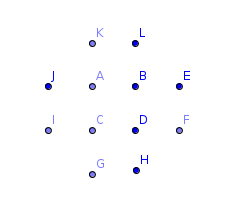
\includegraphics{problema6.png}
    \end{center}
  \end{solucion}

  
  % Un problema de álgebra que mandé a StackExchange
  % ¡Las soluciones podéis mandarlas también allí!
  \begin{enunciado}{Mario Román}{Álgebra}
    Problema escrito en Math.StackExchange:
    \url{http://math.stackexchange.com/questions/633985/is-fn-sum-k-0n-ak-bijective-in-mathbbz-m}
  \end{enunciado}

  % Implementar el KNN
  \begin{enunciado}{Mario Román}{Programación}
    Implementar el algoritmo KNN para clasificación multiclase.
  \end{enunciado}

  % Pequeño problema de invariantes
  \begin{enunciado}{Mario Román}{Coloraciones}
   En cada una de las casillas de una cuadrícula $3 \times 7$ se coloca una ficha azul o una ficha roja.
   Demostrar que siempre podemos encontrar un rectángulo cuyos vértices son cuatro fichas del mismo
   color.
   
   Enunciado de José Miguel Manzano. 
  \end{enunciado}

  % Triángulo de ProjectEuler
  \begin{enunciado}{Marta Andrés}{Programación, Álgebra}
   Enunciado en ProjectEuler: \url{https://projecteuler.net/problem=18} \\
   Enunciado de su generalización en ProjectEuler: \url{https://projecteuler.net/problem=67}
  \end{enunciado}

  % Problema 4 de la OME local edición 46
  
\end{document}